Validation of Napali hinges on the validation of performance of the OPQBoxes. Some of the detection capability of the OPQBoxes has already been characterized as shown in the previous section, however transient response and the $V_{rms}$ response are yet to be confirmed. Once the OPQBox sensitivity has been characterized, the detection capability of Makai system must be crosschecked. First synthetic triggering streams will be injected into Makai. Next the full system will be deployed at the University of Hawaii Manoa for in-situ validation.

\section{OPQBox Validation.}
So far only the frequency sensitivity of the OPQBox has been validated empirically. The transient and as well as $V_{rms}$ response characterization will first be performed using synthetic data. Robust methods for generating power quality events are present in literature, and thus no new research for single device validation is required.\cite{kumar2015power}\cite{tan2013simulation} Next once the DSP software is characterized, synthetic PQ data will be loaded into a SDG1025 signal generator, and fed into the OPQBox hardware. Any discrepancy between the DSP, and hardware-in-the-loop characterization will be noted and analyzed. The main characteristics to be validated are as follows:
\begin{itemize}
  \item{DC response:} Accuracy of the OPQBox in measurement of a DC voltage.
  \item{$V_{rms}$ response:} Accuracy of the OPQBox in measurement of a small changes in the amplitude of AC waveform.
  \item{THD response:} Accuracy of the OPQBox in measurements of small harmonics mixed with a large fundamental AC waveform.
  \item{Transient response:} Validating the response of the OPQBox metrics to various transients.
\end{itemize} 
These tests will provide a baseline for the detection capabilities of the Napali system, and result in a publication regarding the OPQBox detection capabilities.

\section{Makai Synthetic Validation.}
While the synthetic data for a single point PQ disturbance is easily generated, distributed PQ event generation is not well developed. However there is some literature concerning power fault propagation and localization. \cite{parsons1998direction} \cite{polajvzer2017evaluation} The main takeaway from these authors is the energy and amplitude of the event diminishes with electrical distance from the source. As such, by generating a single point PQ event as described in \cite{kumar2015power}\cite{tan2013simulation}, and linearly scaling it based on the simulated electrical distance from the source, a distributed PQ event ensemble can be generated. These events will be ran through the simulated OPQBox DSP stack and the metrics will be propagated to the Makai aggregation sink. Using these events as a baseline, I will be able to tune the threshold and temporal requirements for Makai detection algorithms. Furthermore, temporal, spacial, and amplitude noise will be injected into the generated datasets, to simulate various uncertainties with regards to data collection, such as local noise, and NTP errors. Finally single point PQ events will be injected into Makai to test the local event rejection capabilities.

\section{Napali in-situ Validation}
Once the OPQBox is fully validated and the Makai detection thresholds are tuned using synthetic datasets, the Napali system will be fully deployed at the University of Hawaii at Manoa. In order to validate OPQ system as a whole it will be deployed across the University of Hawaii Manoa campus(UH). This location is ideal because it is a relatively isolated microgrid connected to the Oahu powergrid only via a single 46kV feeder as shown in figure \ref{expdes:fig:1}. Another advantage of the UH campus is the high number of smart meters deployed, across various levels of the power delivery infrastructure. While these meters are mainly geared towards monitoring power consumption they do have some power quality monitoring capabilities. Data provided from these meters can be used in two distinct applications. First of all, this data can be used to pinpoint the section of the University of Hawaii power grid which experience a higher likelihood of power quality disturbances. These portions of the grid will have a higher spacial density of OPQBoxes. Secondly, data from the campus deployed meters can be used as ground truth for comparison against the measurements, and analysis performed by the OPQ project. The location of smart meters in the grid topology is shown in figure \ref{expdes:fig:1} as the $M$ nodes. As evident by the meter location none of them are monitoring the consumer level power and mainly focus on the higher voltage power delivery. This placement is evidenced from the smart meter role as a consumption monitor, and thus the deployment of the OPQBoxes at the residential level will compliment the current power quality monitoring capabilities without introducing redundancies. Finally University of Hawaii powergrid is supplying a highly diverse infrastructure. Beyond the traditional residential equipment such as computers and consumer grade electronics, UH power grid powers scientific and laboratory equipment, machine shops, and server farms. All of these elements have varying requirements/tolerances for power quality anomalies as well as different levels of power quality "pollution". Furthermore some of the electricity consumers in the UH campus is entirely unique. For example the free electron laser located in the Watanabe Hall is one of the only free electron lasers in the world, and the impact/sensitivity of power quality on the instrument are completely unstudied.
\begin{figure}[h]
	\centering
	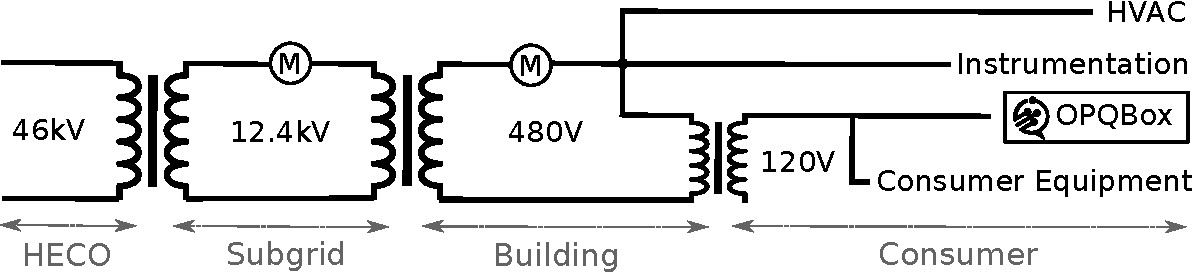
\includegraphics[width=1\linewidth]{img/uh-grid.pdf}	
	\caption{University of Hawaii at Manoa power delivery infrastructure.}
	\label{expdes:fig:3}
\end{figure}
Open power quality project acquired cloud infrastructure from the the Information Technology Services of University of Hawaii, which is hosted on the Manoa campus. This allows for low latency operation, and keeps all of the traffic constrained to the UH internal network. Furthermore UH hosts a Stratum 1 NTP server on its campus. This provides UH OPQ deployment with a low latency, high precision time keeping option. Finally, OPQ project received the Presidents Green Initiative Award in spring 2018. Besides a \$10,000 monetary award, this provides the OPQ project with access to all of the buildings on campus, expertise of the engineers who oversee the campus power infrastructure, as well as access to all of the smart meter measurements already deployed across campus. 

There are 74 smart meters deployed across the UH campus. These meters measure the fundamental frequency $V_{rms}$, power consumption, reactive power, and power factor. Data from these meters will be crossreferenced with the Napali detection system in order to ascertain it's capabilities.

\begin{center}
\begin{tabular}{ ||c | c c|| }
\hline
 \textbf{Activity} & \textbf{Start Date} & \textbf{End Date} \\ 
 \hline
 \hline
 OPQBox2 Validation & October 1\textsuperscript{st} & November 31\textsuperscript{st} \\  
 Makai Validation & October 15 1\textsuperscript{st} & November 30\textsuperscript{th}   \\
 Data Collection & December 1\textsuperscript{st} & TBD   \\
 OPQBox2 Instrumentation paper & January 1\textsuperscript{st} & February 1\textsuperscript{st}   \\
 Data Analysis & February 1\textsuperscript{st} & March 1\textsuperscript{st}  \\
 Introduction Dissertation Chapter & March 1\textsuperscript{st}  & March 15\textsuperscript{th}  \\
 Literature Review Dissertation Chapter & March 15\textsuperscript{th} & April 1\textsuperscript{st}  \\
 Experimental Design Dissertation Chapter & April 1\textsuperscript{st} & April 15\textsuperscript{th}  \\
 Analysis Dissertation Chapter & April 15\textsuperscript{th} & May 15\textsuperscript{th}  \\
 Conclusions Dissertation Chapter & May 15\textsuperscript{th} & June 15\textsuperscript{th}  \\
 \hline
 
\end{tabular}
\end{center}
